\documentclass[10pt,twocolumn]{article}
\usepackage[utf8]{inputenc}
\usepackage[T1]{fontenc}
\usepackage{lmodern}
\usepackage{amsmath,amssymb}
\usepackage{geometry}
\geometry{a4paper,top=2.5cm,bottom=2.5cm,left=2cm,right=2cm,columnsep=0.8cm}
\usepackage{graphicx}
\usepackage{booktabs}
\usepackage{caption}
\usepackage{tikz}
\usepackage{pgfplots}
\pgfplotsset{compat=1.17}
\usetikzlibrary{calc,arrows.meta,positioning,shapes.geometric}
\usepackage{fancyhdr}
\usepackage{lastpage}
\usepackage{xcolor}
\usepackage{mdframed}
\usepackage[authoryear,round]{natbib}
\usepackage{hyperref}
\hypersetup{colorlinks=true,linkcolor=black,citecolor=black,urlcolor=blue}

\pagestyle{fancy}\fancyhf{}
\fancyhead[L]{\small\thepage}
\fancyhead[R]{\small\MakeUppercase{\rightmark}}
\fancyfoot[R]{\small Page \thepage{} / \pageref{LastPage}}
\renewcommand{\headrulewidth}{0pt}\renewcommand{\footrulewidth}{0pt}
\renewcommand{\sectionmark}[1]{\markright{#1}}
\fancypagestyle{firstpage}{\fancyhf{}\fancyhead[L]{\small 1}\fancyhead[R]{\small INNLEIING}\fancyfoot[R]{\small Page 1 / \pageref{LastPage}}\renewcommand{\headrulewidth}{0pt}}

\setlength{\parindent}{1em}\setlength{\parskip}{0pt}
\mdfdefinestyle{abstractbox}{linecolor=black!30,backgroundcolor=black!5,linewidth=0.5pt,innertopmargin=8pt,innerbottommargin=8pt,innerleftmargin=8pt,innerrightmargin=8pt}
\mdfdefinestyle{sidebarbox}{linecolor=black!40,backgroundcolor=black!3,linewidth=0.4pt,innertopmargin=5pt,innerbottommargin=5pt,innerleftmargin=6pt,innerrightmargin=6pt}

\begin{document}
\thispagestyle{firstpage}

\twocolumn[{%
\vspace*{-0.5cm}
\noindent\rule{\textwidth}{0.4pt}\vspace{0.4cm}
{\Large\bfseries Forma som lesbart arkiv: ei Forml\ae re-analyse av \aa tte brettspel\par}\vspace{0.15cm}
{\small Iver Raknes Finne\quad \texttt{iver.raknes.finne@stud.aho.no}\quad AHO\quad \textperiodcentered\quad 2026\par}\vspace{0.5cm}
\begin{mdframed}[style=abstractbox]
\small
\textbf{Samandrag.}\quad Kvifor oppfattar me nokre spel som meir sofistikerte enn andre, gjeve at dei deler same affordansestruktur? Me nyttar Forml\ae re, ein formell designteori som sameinar Stiny sin formgrammatikk (SG), Hatchuel og Weil sin CK-teori, og Levin sitt fleirskalakompetanserammeverk, til \aa{} analysere \aa tte brettspel fr\aa{} tripp-trapp-tresko til Go. Me viser at SG og CK er degenererte spesialtilfelle av Forml\ae re (flatt landskap og triviell grammatikk, respektivt), og at koplingsleddet dei manglar er tilpassingslandskapet kombinert med lyskjegla. Me reformulerer spelaktivitet som ein lyskjegleoperasjon: \aa{} spele er \aa{} utvide eiga prediktive horisont langs speltreet. Arkivdjupna $\mathcal{A}(x) = n_\theta \cdot S$, avleidd fr\aa{} proposisjonane, m\aa ler kor mange motstridande trykk forma samstundes oppretthald gjennom stabiliseringstida. Over \aa tte spel korrelerer $\mathcal{A}$ med BGG-vekt ved Spearman $\rho_s = 0{,}905$ ($p < 0{,}05$); omhugsbreidda $n_\theta$ \aa leine ved $\rho_s = 0{,}929$ ($p < 0{,}01$). Verken SG eller CK kan produsere dette m\aa let \aa leine; Forml\ae re gjer det rutinemessig.
\end{mdframed}
\vspace{0.6cm}
}]


\section{Innleiing}

Kvifor er sjakk ei meir sofistikert form enn dam? Kvifor er Go meir engasjerande enn m\o lle? Kvifor er tripp-trapp-tresko kjedeleg etter ti minutt?

Formgrammatikken \citep{stiny1972,stiny2006} og CK-teorien \citep{hatchuel2003,hatchuel2009} er dei to mest formelt strenge rammeverka i designteori. Begge har generert omfattande forskingslitteratur. Men ingen av dei kan svare p\aa{} desse sp\o rsm\aa la. Grammatikken genererer formelle spr\aa k men rangerer dei ikkje. CK-teorien modellerer designprosessen men har ingen metrikk for produktet. Browne \citep{browne2012} nytta ein simplicity-times-depth-metrikk for speldesign, men utan eit aksiomatisk fundament; Stilman \citep{stilman2000} formaliserte sjakk som lingvistisk geometri utan ein kvalitetsordning. Begge hol er symptom p\aa{} same mangel: inga foreining av syntaks, landskap og agens.

Forml\ae re \citep{finne2026} sameinar dei to tradisjonane med Levin sitt fleirskalakompetanserammeverk \citep{fields2022,doctor2024} i \'ei likning: Form $= SG(\nabla_{C(A)} \mathcal{L}(c,t))$. Grammatikken gjev landskapet formell presisjon; landskapet gjev grammatikken preferansestruktur; lyskjegla $C(A)$ filtrerer kva trykk som blir representerte. Saman produserer dei eit kvalitetsm\aa l ingen av delane har \aa leine.

Me vel bevisst ein artefaktklasse der intuisjonen er sterk, affordansestrukturen er identisk, og uavhengige data er tilgjengelege. Me analyserer \aa tte brettspel fr\aa{} tripp-trapp-tresko ($10^3$ tilstandar) til Go ($10^{170}$), og samanliknar formelle arkivskårar med brukardata fr\aa{} BoardGameGeek (BGG). Testtilfellet er designa for \aa{} vere lett \aa{} falsifisere: dersom apparatet ikkje kan fange skilnaden me alle opplever, generaliserer det ikkje. Dersom det kan, har me grunn til \aa{} tru at same apparat, allereie validert mot 2\,066 materielle artefaktar (stolar; \citealp{finne2026}), ogs\aa{} fungerer for abstrakte.

Bidraget er firedelt: (1)~ein demonstrasjon av at SG og CK er degenererte spesialtilfelle av Forml\ae re; (2)~ein reformulering av spelaktivitet som lyskjegleoperasjon; (3)~ein formell arkivdjupn-indeks $\mathcal{A}$ avleidd fr\aa{} proposisjonane; (4)~ein empirisk korrelasjon over \aa tte spel ($\rho_s = 0{,}905$).


\section{Relatert arbeid}

Spelkompleksitetsteori \citep{shannon1950,allis1994,vandenherik2002,schaeffer2007,takizawa2023} kvantifiserer speltre og tilstandsrom men definerer ikkje arkivdjupn; eit spel kan ha h\o g kompleksitet utan \aa{} vere lesbart. Browne og Maire \citep{browne2010}, Browne \citep{browne2012} og Ludii-gruppa \citep{piette2020} utvikla induktive metrikkar for speldesignkvalitet utan formelt fundament. Stilman \citep{stilman2000} formaliserte strategiske spel som lingvistisk geometri men kunne ikkje rangere. Dormans \citep{dormans2010} nytta formgrammatikkar p\aa{} videospel-niv\aa design, ikkje regelsystem. MDA \citep{hunicke2004}, spel-ontologien \citep{zagal2005} og Elias et al.\ \citep{elias2012} kartlegg komponentar utan \aa{} foreine dei. Forml\ae re gjev fundamentet som manglar.


\section{SG og CK som degenererte tilfelle}

Ein formgrammatikk $SG = (S, R, \omega)$ for eit brettspel har stillingar~$S$, lovlege trekk $R$ (regel $r_i$ gjenkjenner m\o nster $\tau(a_i) \leq s$ og transformerer $s \to (s - \tau(a_i)) + \tau(b_i)$), og startstilling~$\omega$. For sjakk har $R$ seks distinkte r\o rslemodular; for tripp-trapp-tresko \'ein. Spr\aa ka $L(SG)$ varierer over 89 storleiksordnar, men grammatikken skil ikkje mellom dei. Han er n\o ytral til kvalitet.

CK-teorien navigerer kunnskapsrom $K$ og tankerom $C$ gjennom fire operat\o rar (figur~\ref{fig:cksquare}). Men $C$ manglar geometrisk struktur \citep{coatanea2010}; han modellerer \textit{prosessen} men ikkje \textit{produktet}.

\begin{figure}[t]
\centering
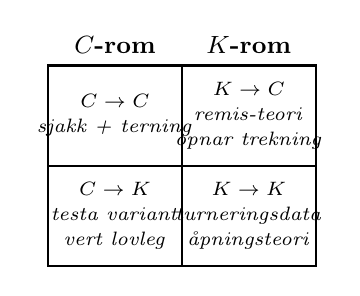
\begin{tikzpicture}[scale=0.85,font=\scriptsize]
\draw[thick] (0,0) rectangle (4,3);
\draw[thick] (2,0) -- (2,3);
\draw[thick] (0,1.5) -- (4,1.5);
\node[font=\bfseries\small] at (1,3.3) {$C$-rom};
\node[font=\bfseries\small] at (3,3.3) {$K$-rom};
\node[align=center] at (1,2.25) {$C \to C$\\[1pt]\textit{sjakk + terning}};
\node[align=center] at (3,2.25) {$K \to C$\\[1pt]\textit{remis-teori}\\[1pt]\textit{opnar trekning}};
\node[align=center] at (1,0.75) {$C \to K$\\[1pt]\textit{testa variant}\\[1pt]\textit{vert lovleg}};
\node[align=center] at (3,0.75) {$K \to K$\\[1pt]\textit{turneringsdata}\\[1pt]\textit{\aa pningsteori}};
\end{tikzpicture}
\caption{CK Design Square med sjakk som d\o me. Fire operat\o rar navigerer mellom tankerom $C$ og kunnskapsrom $K$. CK-teorien formaliserer navigasjonen men gjev ingen kvalitetsm\aa l for endepunktet.}
\label{fig:cksquare}
\end{figure}

Forml\ae re gjev $C$ geometri gjennom formrommet~$M$, legg til tilpassingslandskapet~$\mathcal{L}$, og lyskjegla~$C(A)$. Kjernelikninga Form $= SG(\nabla_{C(A)} \mathcal{L}(c,t))$ inneheld begge tradisjonane som degenererte tilfelle. Sett $\nabla \mathcal{L} = 0$: likninga reduserer til Form $= SG(0)$, grammatikken utan preferanse. Sett $SG$ triviell: likninga reduserer til Form $= \nabla_{C(A)} \mathcal{L}$, CK-navigasjon utan $C$-geometri. Forml\ae re er ikkje eit alternativ men ein sameining; meirverdien er koplingsleddet.


\section{Spel som lyskjegleoperasjon}

\AA{} spele er ikkje berre \aa{} f\o lgje grammatikken; det er \aa{} simulere motstandaren. Ein kompetent spelar held fleire trekk framover representert samstundes, evaluerer stillingane dei leier til, og vel den som maksimerer eigne utfall under antatt motspel. Dette er ein lyskjegleoperasjon i Levin og Fields si forstand \citep{fields2022}: agenten utvidar si eiga prediktive horisont langs speltreet, og trekkjer berre det trekket som minimaliserer forventa fri-energi over horisonten \citep{friston2010,pezzulo2015}.

Operasjonen er ikkje ny; ho er pavlovsk betinging iterert og akkumulert. Hjernen lagrar kondisjonerte stimulus som prediksjonsverdiar (traktaten, prop.\ 10); speltreet er ein strukturert katalog av slike prediksjonar. Bayesiansk theory-of-mind \citep{baker2011} formaliserer modelleringa av motstandaren som ein inferens over skjult preferanse. Empirisk viser Haworth et al.\ \citep{haworth2010} at sjakkspelarar er Bayesianske prediktorar: feilvalg ber m\aa lbar distribusjon som f\o lgjer kompetanseniv\aa{} monotont.

Forml\ae re-konsekvensen: omhugsbreidda $n_\theta$ m\aa ler sjangerbreidda agenten m\aa{} oppretthalde i lyskjegla si for \aa{} spele kompetent. Eit spel som forl\o yser seks trykk samstundes (sjakk, Go) krev at ein kompetent spelar balanserer seks aksar prediktivt; eit spel som forl\o yser to (dam, tripp-trapp-tresko) krev to. Skilnaden mellom sjakk og dam er ikkje \guillemotleft djupn\guillemotright{} i abstrakt forstand; han er eit objektivt lyskjegle-volum.

Figur~\ref{fig:lightcone} viser denne kontrasten. Dam sin smale kjegle sviktar systematisk langs aksane Drama, Prestige og Materiell differensiering (flate strategiske sluttspel; marginal kulturell kanon; to identiske brikketypar). Sjakk sin breie kjegle realiserer alle seks. Svikt-signaturen er ikkje tilfeldig; han er forma si lesbare arkiv av kva trykk som vart ignorerte.

\begin{figure}[t]
\centering
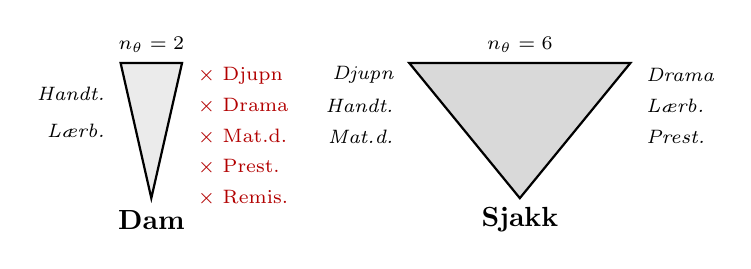
\begin{tikzpicture}[scale=0.78,font=\scriptsize]
\draw[thick,fill=black!8] (0,0) -- (-0.5,2.2) -- (0.5,2.2) -- cycle;
\node[font=\bfseries] at (0,-0.35) {Dam};
\node[font=\scriptsize] at (0,2.5) {$n_\theta = 2$};
\node[anchor=east,font=\scriptsize\itshape] at (-0.6,1.7) {Handt.};
\node[anchor=east,font=\scriptsize\itshape] at (-0.6,1.1) {L\ae rb.};
\node[anchor=west,font=\scriptsize,red!70!black] at (0.6,2.0) {$\times$ Djupn};
\node[anchor=west,font=\scriptsize,red!70!black] at (0.6,1.5) {$\times$ Drama};
\node[anchor=west,font=\scriptsize,red!70!black] at (0.6,1.0) {$\times$ Mat.d.};
\node[anchor=west,font=\scriptsize,red!70!black] at (0.6,0.5) {$\times$ Prest.};
\node[anchor=west,font=\scriptsize,red!70!black] at (0.6,0.0) {$\times$ Remis.};
\begin{scope}[xshift=6cm]
\draw[thick,fill=black!15] (0,0) -- (-1.8,2.2) -- (1.8,2.2) -- cycle;
\node[font=\bfseries] at (0,-0.35) {Sjakk};
\node[font=\scriptsize] at (0,2.5) {$n_\theta = 6$};
\node[anchor=east,font=\scriptsize\itshape] at (-1.9,2.0) {Djupn};
\node[anchor=east,font=\scriptsize\itshape] at (-1.9,1.5) {Handt.};
\node[anchor=east,font=\scriptsize\itshape] at (-1.9,1.0) {Mat.d.};
\node[anchor=west,font=\scriptsize\itshape] at (1.9,2.0) {Drama};
\node[anchor=west,font=\scriptsize\itshape] at (1.9,1.5) {L\ae rb.};
\node[anchor=west,font=\scriptsize\itshape] at (1.9,1.0) {Prest.};
\end{scope}
\end{tikzpicture}
\caption{Lyskjegler og svikt-signaturar. Dam realiserer to av sju seleksjonstrykk; dei fem urepresenterte aksane ($\times$) utgjer svikt-signaturen. Sjakk realiserer seks. Breidda er ikkje subjektiv; ho er telt fr\aa{} operasjonaliserte trykk.}
\label{fig:lightcone}
\end{figure}


\section{Formrom og kvantitative data}

\begin{table*}[t]
\centering\small
\caption{Formromsdata for \aa tte spel. Tilstandsrom og speltre: $\log_{10}$. $b$: forgreiningsfaktor. $H = \log_2 b$ (bit/trekk). Kjelder: Allis (1994), BGG, solved-games-kanon.}
\label{tab:formrom}
\begin{tabular}{@{}lccccccccl@{}}
\toprule
Spel & Tilstandsrom & Speltre & $b$ & $H$ & Mod. & L\o yst? & $\Delta t$ (\aa r) & BGG-vekt & BGG-vurd. \\
\midrule
Tripp-trapp-tresko & 3 & 5 & 4 & 2,0 & 1 & Ja (triv.) & $-$ & 1,1 & 3,3 \\
Connect Four & 12 & 21 & 4 & 2,0 & 1 & Ja (1988) & 14 & 1,2 & 5,4 \\
M\o lle & 10 & 50 & 10 & 3,3 & 2 & Ja (1993) & ${\sim}1000$ & 1,8 & 5,2 \\
Dam & 20 & 40 & 2,8 & 1,5 & 2 & Ja (2007) & ${\sim}500$ & 1,8 & 4,6 \\
Othello & 28 & 58 & 10 & 3,3 & 1 & Ja (2023) & 46 & 2,1 & 5,8 \\
Backgammon & 20 & 144 & 250 & 8,0 & 3 & Nei & ${\sim}5000$ & 2,4 & 6,9 \\
Sjakk & 44 & 123 & 35 & 5,1 & 6 & Nei & ${\sim}550$ & 3,7 & 6,9 \\
Go & 170 & 505 & 250 & 8,0 & 1 & Nei & ${\sim}4000$ & 4,0 & 7,6 \\
\bottomrule
\end{tabular}
\end{table*}

Tabell~\ref{tab:formrom} viser ni kvantifiserbare formromsparametrar for alle \aa tte spel. Merk at $\Delta t$ for l\o yste spel er \aa r fr\aa{} etablert konkurransetradisjon til l\o ysing; for ul\o yste, \aa r med aktiv tradisjon.

\begin{mdframed}[style=sidebarbox]
\small\textbf{Datahistorie som stresstest.}\quad L\o ysingstidspunktet korrelerer lite med arkivdjupna. Connect Four l\o yst 1988 \citep{allis1994}; dam 2007 \citep{schaeffer2007}; Othello 2023 \citep{takizawa2023}. Deep Blue overgjekk Kasparov i 1997 utan at sjakk er l\o yst. AlphaZero \citep{silver2018} og MuZero l\ae rer regelsett sj\o lv utan at Go er l\o yst. Computationell gjennombrot endrar ikkje forma sitt arkiv; dei endrar kven som kan lese det. Backgammon er ul\o yst, men har BGG-vekt 2,4: terningane maskerer dei $10^{144}$ speltre-posisjonane for folkem\aa let. $\mathcal{A}$ ser gjennom maskeringa ($\mathcal{A} = 22{,}2$).
\end{mdframed}


\section{Seleksjonstrykk}

For kvart spel identifiserer me sju seleksjonstrykk (tabell~\ref{tab:omhug}): tre kvantifiserbare ($P_1$~Djupn, $P_2$~Handterlegheit, $P_3$~Materiell differensiering), fire operasjonaliserte ($P_4$~Drama, stillingssvingingar siste 30 trekk; $P_5$~L\ae rbarheit, timar til kompetanse; $P_6$~Prestige, kulturell institusjonalisering; $P_7$~Remisrate). Omhugsbreidda $n_\theta = |\{i : r_i > \theta\}|$ med $\theta = 0{,}5$ varierer fr\aa{} 2 til 6. Spel med l\aa g $n_\theta$ sviktar systematisk langs dei urepresenterte aksane, n\o yaktig slik proposisjon~7 predikerer.

\begin{table}[t]
\centering\scriptsize
\caption{Omhugsprofil for \aa tte spel. $\theta = 0{,}5$. Siste rad: $n_\theta$ og $\bar{r}$.}
\label{tab:omhug}
\begin{tabular}{@{}lcccccccc@{}}
\toprule
& TT & C4 & M\o & Da & Ot & Bg & Sj & Go \\
\midrule
$P_1$ Djupn & .05 & .25 & .45 & .25 & .55 & .60 & .95 & .99 \\
$P_2$ Handt. & .99 & .95 & .80 & .95 & .80 & .70 & .75 & .60 \\
$P_3$ Mat.d. & .05 & .05 & .20 & .10 & .10 & .30 & .90 & .05 \\
$P_4$ Drama & .05 & .20 & .30 & .15 & .65 & .80 & .85 & .75 \\
$P_5$ L\ae rb. & .95 & .90 & .85 & .70 & .85 & .75 & .80 & .70 \\
$P_6$ Prest. & .05 & .10 & .15 & .20 & .35 & .55 & .70 & .65 \\
$P_7$ Remis. & .05 & .70 & .10 & .10 & .90 & .95 & .30 & .90 \\
\midrule
$n_\theta$ & 2 & 3 & 2 & 2 & 5 & 6 & 6 & 6 \\
$\bar{r}$ & .31 & .45 & .41 & .35 & .60 & .66 & .75 & .66 \\
\bottomrule
\end{tabular}
\end{table}


\section{Arkivdjupn}

\subsection{Avleiing fr\aa{} proposisjonane}

Arkivdjupn spring fr\aa{} to proposisjonar. Proposisjon~7 seier at den realiserte forma er eit leseleg arkiv over kompromisset sin dimensjonalitet: forma viser kor mange motstridande seleksjonstrykk agenten aktivt representerte. Mengda av forl\o yste trykk er omhugsbreidda $n_\theta(x) = |\{i : r_i(x) > \theta\}|$.

Proposisjon~3 seier at stabiliteten til ei form svarar til brattleiken p\aa{} dalveggane i tilpassingslandskapet: kanalisering. Me operasjonaliserer kanaliseringsdjupna som $S(x) = \log_{10}(\Delta t)$, der $\Delta t$ er konkurranselevetida i \aa r.

Arkivdjupna er koplingsproduktet:
\begin{equation}
\mathcal{A}(x) = n_\theta(x) \cdot S(x)
\end{equation}

Produktforma er ikkje vilk\aa rleg. Omhugsbreidde utan stabilitet er skj\o rheit; stabilitet utan omhugsbreidde er primitivitet. Sumforma $n_\theta + S$ ville tillate kompensasjon: eit spel stabilt i tusen \aa r men med berre eitt trykk ville sk\aa re h\o gt. Produktet avviser dette.

Browne \citep{browne2012} definerte eleganse som simplicity-times-depth. Arkivdjupn er formelt annleis: $\mathcal{A}$ m\aa ler dimensjonsbreidde gonger temporal kanalisering, ikkje invers kompleksitet gonger strategisk djupn. Dei to metrikkane gjev lik ordning for dei fire klassiske spela sjakk, dam, Go, Othello, men avvik for backgammon, der Browne-metrikken straffar terning-st\o y medan $\mathcal{A}$ premierer den strategiske djupna under st\o yen.

\subsection{Ekstern validering}

Arkivdjupna er robust mot parameterval: sjakk rangerer over dam ved $\theta \in \{0{,}4; 0{,}5; 0{,}6\}$ og ved $\pm 0{,}15$ forstyrring av $P_4$--$P_6$ i worst-case-retning.

Figur~\ref{fig:scatter} viser hovudresultatet. Over \aa tte spel korrelerer $\mathcal{A}$ med BGG-vekt ved Spearman $\rho_s = 0{,}905$ ($p < 0{,}05$, kritisk verdi 0,738 for $n = 8$). Omhugsbreidda $n_\theta$ \aa leine korrelerer ved $\rho_s = 0{,}929$ ($p < 0{,}01$). Gjennomsnittleg forl\o ysingsgrad $\bar{r}$ korrelerer ved $\rho_s = 0{,}881$.

\begin{figure}[t]
\centering
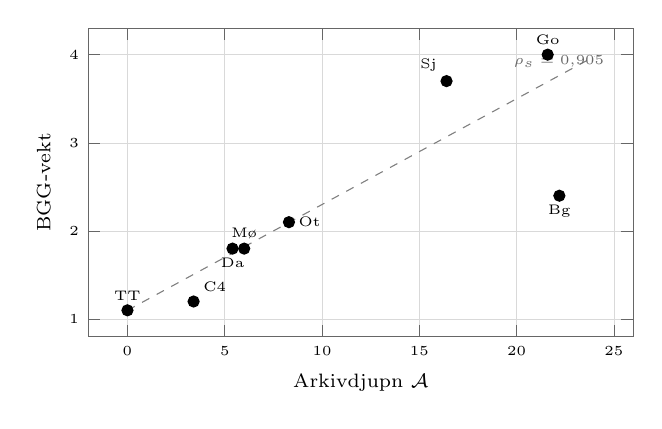
\begin{tikzpicture}[font=\scriptsize]
\begin{axis}[
    width=8.5cm,height=5.5cm,
    xlabel={Arkivdjupn $\mathcal{A}$},
    ylabel={BGG-vekt},
    xmin=-2,xmax=26,ymin=0.8,ymax=4.3,
    xtick={0,5,10,15,20,25},
    ytick={1,2,3,4},
    grid=major,grid style={black!15,very thin},
    axis line style={black!60},
    tick style={black!60},
    label style={font=\scriptsize},
    tick label style={font=\tiny},
]
\addplot[only marks,mark=*,mark size=2pt,black] coordinates {
    (0,1.1) (3.4,1.2) (5.4,1.8) (6.0,1.8) (8.3,2.1) (16.4,3.7) (21.6,4.0) (22.2,2.4)
};
\node[anchor=south,font=\tiny] at (axis cs:0,1.1) {TT};
\node[anchor=south west,font=\tiny] at (axis cs:3.4,1.2) {C4};
\node[anchor=north,font=\tiny] at (axis cs:5.4,1.8) {Da};
\node[anchor=south,font=\tiny] at (axis cs:6.0,1.8) {M\o};
\node[anchor=west,font=\tiny] at (axis cs:8.3,2.1) {Ot};
\node[anchor=south east,font=\tiny] at (axis cs:16.4,3.7) {Sj};
\node[anchor=south,font=\tiny] at (axis cs:21.6,4.0) {Go};
\node[anchor=north,font=\tiny] at (axis cs:22.2,2.4) {Bg};
\addplot[dashed,black!50,thin,domain=0:24] {1.1 + 0.12*x};
\node[anchor=north east,font=\tiny,black!60] at (axis cs:25,4.1) {$\rho_s = 0{,}905$};
\end{axis}
\end{tikzpicture}
\caption{Arkivdjupn $\mathcal{A}$ mot BGG-vekt over \aa tte spel. Spearman $\rho_s = 0{,}905$ ($p < 0{,}05$); $n_\theta$ \aa leine $\rho_s = 0{,}929$ ($p < 0{,}01$). Backgammon (Bg) er det einaste avviket: $\mathcal{A}$ ser gjennom terning-maskering av strategisk djupn.}
\label{fig:scatter}
\end{figure}

Korrespondansen krev varsam tolking. BGG-vurderingar reflekterer ogs\aa{} kulturell prestisje, nostalgi og sj\o lvseleksjon. Tre observasjonar styrkar likevel korrespondansen. For det f\o rste: BGG-vekt m\aa ler opplevd kompleksitet snarare enn preferanse, og er mindre utsett for kulturell bias. For det andre: $\mathcal{A}$ forklarer kvifor backgammon avvik fr\aa{} trenden; det sk\aa rar h\o gare p\aa{} $\mathcal{A}$ (22,2) enn BGG-vekt (2,4), fordi terningane maskerer den reelle strategiske djupna. For det tredje: $n_\theta$ korrelerer sterkare med BGG-vurdering ($\rho_s = 0{,}976$) enn med BGG-vekt ($\rho_s = 0{,}929$), noko som tyder p\aa{} at omhugsbreidda fangar ein dimensjon av opplevd kvalitet utover rein kompleksitet.

\begin{table}[h]
\centering\small
\caption{Arkivdjupn og BGG-data, sortert etter $\mathcal{A}$.}
\label{tab:results}
\begin{tabular}{@{}lcccc@{}}
\toprule
Spel & $n_\theta$ & $S$ & $\mathcal{A}$ & BGG-vekt \\
\midrule
Tripp-trapp-tresko & 2 & 0 & 0 & 1,1 \\
Connect Four & 3 & 1,2 & 3,4 & 1,2 \\
Dam & 2 & 2,7 & 5,4 & 1,8 \\
M\o lle & 2 & 3,0 & 6,0 & 1,8 \\
Othello & 5 & 1,7 & 8,3 & 2,1 \\
Sjakk & 6 & 2,7 & 16,4 & 3,7 \\
Go & 6 & 3,6 & 21,6 & 4,0 \\
Backgammon & 6 & 3,7 & 22,2 & 2,4 \\
\bottomrule
\end{tabular}
\end{table}


\section{Falsifiseringsvilk\aa r}

(a)~Eit spel med l\aa g $n_\theta$ presterer like godt som eit med h\o g $n_\theta$ langs dei same aksane: omhugsdiagnosen falsifisert. (b)~$\rho_s(\mathcal{A}, \text{BGG-vekt})$ er ikkje signifikant ved replikasjon med andre spel: indeksen falsifisert. (c)~Spelarar vurderer dam som meir sofistikert enn sjakk i kontrollerte eksperiment: analysen falsifisert. (d)~CK- eller SG-rammeverk produserer arkivdjupn-ekvivalent metrikk utan Forml\ae re-koplingsleddet: foreinings-p\aa standen falsifisert.


\section{Konklusjon}

Formgrammatikken og CK-teorien er begge degenererte spesialtilfelle av Forml\ae re. Grammatikken genererer utan preferanse; CK-teorien navigerer utan formell geometri. Forml\ae re legg til koplingsleddet: tilpassingslandskapet $\mathcal{L}$ som favoriserer visse former, og lyskjegla $C(A)$ som avgjer kva trykk agenten representerer. Spelaktivitet er sj\o lv ein lyskjegleoperasjon: \aa{} spele er \aa{} halde prediktive horisontar over speltreet opne. Ein sameint teori seier minst like mykje som dei to kvar for seg, og meir.

Over \aa tte brettspel fr\aa{} tripp-trapp-tresko til Go korrelerer arkivdjupna $\mathcal{A}$ med uavhengige BGG-data ved $\rho_s = 0{,}905$. M\o nsteret er konsistent: spel der regelsettet navigerer mange motstridande trykk samstundes (h\o g $n_\theta$) vert oppfatta som meir sofistikerte. Spel der regelsettet berre forl\o yser f\aa{} trykk sviktar langs dei urepresenterte aksane: dam er strategisk utt\o mt, tripp-trapp-tresko er narrativt tomt, m\o lle er materielt monotont.

Arkivdjupn er ein formell eigenskap ved forma. Forma viser kor langt omhugen rakk.


\small
\subsection*{Referansar}
\begingroup\renewcommand{\section}[2]{}
\begin{thebibliography}{99}\small
\bibitem[Allis(1994)]{allis1994} Allis, V. (1994). \textit{Searching for Solutions in Games and AI.} PhD, U.\ Limburg.
\bibitem[Baker et al.(2011)]{baker2011} Baker, C., Saxe, R., Tenenbaum, J. (2011). Bayesian theory of mind: Modeling joint belief-desire attribution. \textit{Proc.\ CogSci}.
\bibitem[Browne \& Maire(2010)]{browne2010} Browne, C., Maire, F. (2010). Evolutionary game design. \textit{IEEE Trans.\ Comp.\ Intell.\ AI in Games}, 2(1), 1--16.
\bibitem[Browne(2012)]{browne2012} Browne, C. (2012). Elegance in game design. \textit{IEEE Trans.\ Comp.\ Intell.\ AI in Games}, 4(3), 229--240.
\bibitem[Coatan\'ea et al.(2010)]{coatanea2010} Coatan\'ea, E.\ et al.\ (2010). CK theory: Contributions and limits. \textit{Proc.\ DETC}, 83--92.
\bibitem[Doctor et al.(2024)]{doctor2024} Doctor, T.\ et al.\ (2024). Care as the driver of intelligence. \textit{Entropy}, 26(4), 352.
\bibitem[Dormans(2010)]{dormans2010} Dormans, J. (2010). Adventures in level design: generating missions and spaces for action adventure games. \textit{Proc.\ PCG Workshop, FDG}.
\bibitem[Elias et al.(2012)]{elias2012} Elias, G.\ S., Garfield, R., Gutschera, K.\ R. (2012). \textit{Characteristics of Games.} MIT Press.
\bibitem[Fields \& Levin(2022)]{fields2022} Fields, C., Levin, M. (2022). Competency in navigating arbitrary spaces. \textit{Entropy}, 24(6), 819.
\bibitem[Finne(2026)]{finne2026} Finne, I.\ R. (2026). Form som arkiv av omhug. Arbeidspapir, AHO.
\bibitem[Friston(2010)]{friston2010} Friston, K. (2010). The free-energy principle: A unified brain theory? \textit{Nat.\ Rev.\ Neurosci.}, 11, 127--138.
\bibitem[Hatchuel \& Weil(2003)]{hatchuel2003} Hatchuel, A., Weil, B. (2003). A new approach of innovative design: an introduction to CK theory. \textit{Proc.\ ICED}.
\bibitem[Hatchuel \& Weil(2009)]{hatchuel2009} Hatchuel, A., Weil, B. (2009). C-K design theory: An advanced formulation. \textit{Res.\ Eng.\ Des.}, 19(4), 181--192.
\bibitem[Haworth et al.(2010)]{haworth2010} Haworth, G., Regan, K., Di Fatta, G. (2010). Performance and prediction: Bayesian modelling of fallible choice in chess. \textit{Advances in Computer Games}, LNCS 6048, Springer, 99--110.
\bibitem[Hunicke et al.(2004)]{hunicke2004} Hunicke, R., LeBlanc, M., Zubek, R. (2004). MDA: A formal approach to game design and game research. \textit{Proc.\ AAAI Workshop on Challenges in Game AI}.
\bibitem[Pezzulo et al.(2015)]{pezzulo2015} Pezzulo, G., Rigoli, F., Friston, K. (2015). Active inference, homeostatic regulation and adaptive behavioural control. \textit{Prog.\ Neurobiol.}, 134, 17--35.
\bibitem[Piette et al.(2020)]{piette2020} Piette, \'E.\ et al.\ (2020). Ludii: The ludemic general game system. \textit{Proc.\ ECAI}, 411--418.
\bibitem[Schaeffer et al.(2007)]{schaeffer2007} Schaeffer, J.\ et al.\ (2007). Checkers is solved. \textit{Science}, 317, 1518--1522.
\bibitem[Shannon(1950)]{shannon1950} Shannon, C. (1950). Programming a computer for chess. \textit{Phil.\ Mag.}, 41(314), 256--275.
\bibitem[Silver et al.(2018)]{silver2018} Silver, D.\ et al.\ (2018). A general reinforcement learning algorithm that masters chess, shogi, and Go. \textit{Science}, 362, 1140--1144.
\bibitem[Stilman(2000)]{stilman2000} Stilman, B. (2000). \textit{Linguistic Geometry: From Search to Construction.} Kluwer.
\bibitem[Stiny \& Gips(1972)]{stiny1972} Stiny, G., Gips, J. (1972). Shape grammars. \textit{Inf.\ Proc.\ 71}, 1460--1465.
\bibitem[Stiny(2006)]{stiny2006} Stiny, G. (2006). \textit{Shape.} MIT Press.
\bibitem[Takizawa(2023)]{takizawa2023} Takizawa, H. (2023). Othello is solved. Preprint, arXiv:2310.19387.
\bibitem[Van den Herik et al.(2002)]{vandenherik2002} Van~den~Herik, H.\ J.\ et al.\ (2002). Games solved: Now and in the future. \textit{Artif.\ Intell.}, 134, 277--311.
\bibitem[Zagal et al.(2005)]{zagal2005} Zagal, J.\ P.\ et al.\ (2005). Towards an ontological language for game analysis. \textit{Proc.\ DiGRA}.
\end{thebibliography}
\endgroup

\end{document}
